% .:: Laden der LaTeX4EI Formelsammlungsvorlage
\documentclass[european]{latex4ei_sheet}

\title{Elektrische \\ Energietechnik}

\RequirePackage{latex4ei/latex4ei_unicode}

% DOCUMENT_BEGIN ===============================================================
\begin{document}

\IfFileExists{git.id}{\input{git.id}}{}
\ifdefined\GitRevision\mydate{\GitNiceDate\ (git \GitRevision)}\fi

% Title (needs ./img/Logo.pdf)
\maketitle

% ---------------------------------------
% | 		Energietechnik	 			|
% ~~~~~~~~~~~~~~~~~~~~~~~~~~~~~~~~~~~~~~~
%=======================================================================

	\section{Physikalische Grundlagen}
	$P = F \cdot v = M \cdot \omega$ \\
	Kreisfrequenz: $\omega := \frac{\diff \phi}{\diff t} = 2 \pi n = 2 \pi f = \frac{v}{r}$ \\
	\section{Lastganglinien}
	$T_n$: Nennbetriebsdauer\\
	$T_a$ Ausnutzungsadauer\\
	$T_{ben}$: Benutzungsdauer\\
	$P_{max}$: Höchstalast\\
	$W = \int_0^{T_n} P(t) \diff t = P_{mittel} T_n = P_n T_a = P_{max} T_{ben}$\\
	\section{Wechsel-/Drehstromsystem}
		\subsection{Wechselstromsystem}
		Phasenwinkel: $\varphi = \varphi_u - \varphi_i$ \qquad Scheitelwert: $\hat x$\\
		Effektivwert: $X=\frac{\hat x}{\sqrt{2}} = \sqrt{\frac{1}{T} \int_{t_0}^{t_0 + T} x^2(\tau) \diff \tau}$\\
		Zeitsignal: $x(t) = \hat x \cos(\omega t + \varphi_x) = X \sqrt{2} \cos(\omega t + \varphi_x)$\\
		Komplexes Zeitsignal: $\vec x(t) = \hat x \exp\left[\j (\omega t + \varphi_x)\right]$\\ 
		mit \qquad \qquad $x(t) = \Re{\vec x(t)}$

		Effektiver Zeiger: $\vec X = X \exp(\j \varphi_x) =\frac{1}{\sqrt{2} \exp(\j \omega t)}\vec x(t)$\\
		\subsection{Komplexe Leistung}
		$P = \frac1T \int_0^{T} p(t) \diff t = \frac1T \int_0^{T} u(t) \cdot i(t) \diff t$\\
		$p(t) = P + S \cdot \cos(2\omega t + \varphi_u + \varphi_i)$\\
		\begin{symbolbox}
			\begin{tabular}{lll}
				Wirkleistung & $P = \Re{\vec S} = U I \cdot \cos(\varphi)$ & $\si{W}$\\
				Blindleistung & $Q = \Im{\vec S} = U I \cdot \sin(\varphi)$ & $\si{Var}$\\
				Scheinleistung & $S = \norm{\vec U \cdot \vec I^*} = \sqrt{P^2 + Q^2}$ & $\si{VA}$\\
			\end{tabular}
		\end{symbolbox}
		Leistungsfaktor $\lambda = \frac{|P|}{S} = \cos(\varphi)$ \qquad
		\includegraphics[scale=1]{./img/leistung.pdf}\\
		
		Scheinleistung schwingt mit doppelter Netzfrequenz!\\
		Komplexe Wechselleistung: $\tilde {\vec S} = \vec U \cdot \vec I$\\

		\begin{tablebox}{ll}
		Impedanz(Scheinwiderstand) & Admittanz(Scheinleitwert)\\
		\mrule
		$\vec Z = R + \j X = \exp(\j \varphi_Z)$ & $\vec Y = G + \j B = \exp(\j \varphi_Y)$\\
		$\underset{\text{Impedanz}}{Z(j\omega)} = \underset{\text{Resistanz}}{R(j\omega)} + \underset{\text{Reaktanz}}{jX(j\omega)}$ & 	$\underset{\text{Admittanz}}{Y(j\omega)} = \underset{\text{Konduktanz}}{G(j\omega)} + \underset{\text{Suszeptanz}}{jB(j\omega)}$\\
		$\vec U = \vec Z \cdot I $ & $\vec I = \vec Y \cdot \vec U$\\

		\end{tablebox}



		\subsection{Drehstromsystem}
		Drehoperator: $\vec a = \exp\bigl(\j \frac{2}{3} \pi \bigr)$ \qquad $\vec a^0 = \vec a^3 = 1$ \quad $\vec a^* = \vec a^2$\\
		
		% Zeigerdiagramm mit Drehoperatoren
		
		Effektive Leiter-Erdspannungen: $\vec U_1,\vec U_2,\vec U_3$\\
		Effektive Außenleiterspannungen: $\vec U_{12},\vec U_{23},\vec U_{31}$\\
		Netznennspannung: $U_n$\\
		
		
		\begin{tablebox}{lll}
			symmetrisch & unsymmetrisch\\
			$U = |U_1| = |U_2| = |U_3|$ & \\
		 	$U_n = |U_{12}| = |U_{23}| = |U_{32}| = \sqrt{3} U$ & \\
		 	$\vec S = 3 \cdot \vec U\vec I^*$ & $\vec S = \sum_{k=1}^3\vec U_k\vec I_k^\star$\\
		\end{tablebox}
		
		Komplexe Wechselleistung: $\tilde{\vec S} = \vec U_1 \cdot \vec I_1 + \vec U_2 \cdot \vec I_2 + \vec U_3 \cdot \vec I_3$
		Tatsächlicher Leistungsfluss: $p(t) = \operatorname{Re} \left\{ \vec S \right\} + \operatorname{Re} \left\{\tilde{\vec S} e^{j 2 \omega t} \right\}$
	\subsection{Sternschaltung}
	Falls symmetrisch gilt:\\
	 $\vec I = \abs{\vec I_1} = \abs{\vec I_2} = \abs{\vec I_3}$, $\vec U = \abs{\vec U_1} = \abs{\vec U_2} = \abs{\vec U_3}$ und $I=\frac{U}{\abs Z}$
	\subsection{Dreieckschaltung}
	Eine symmetrische Dreiecksschaltung kann durch eine Sternschaltung mit $\vec Z_*=1/3 \cdot \vec Z_\Delta$ ersetzt werden.\\
	Falls symmetrisch gilt:\\
	$\vec I_\Delta = \abs{\vec I_{12}} = \abs{\vec I_{23}} = \abs{\vec I_{31}}$, $\vec U_\Delta = \abs{\vec U_{12}} = \abs{\vec U_{23}} = \abs{\vec U_{31}}$ und $I_\Delta=\frac{U_n}{\abs Z}$
	\subsection{Impedanzmatrix}
	\[\begin{pmatrix} \vec U_1 \\ \vec U_2 \\ \vec U_3 \end{pmatrix} = 
		\begin{pmatrix} \vec A & \vec B & \vec B \\ \vec B & \vec A & \vec B \\ \vec B & \vec B & \vec A \end{pmatrix} 
		\begin{pmatrix} \vec I_1 \\ \vec I_2 \\ \vec I_3 \end{pmatrix}\]
		Eigenimpedanz: $\vec A$, Koppelimpedanz: $\vec B$\\
		Betriebsimpedanz $\vec Z_b = \vec A - \vec B$

	\section{Elektrische Maschinen}
	sind Betriebsmittel, welche Energie mittels eines Feldes wandeln. Man unterscheidet ruhende elektrische Maschinen (Trafo) und rotierende elektrische Maschinen (Generator, Motor, Umformer)
		\subsection{Der Transformator}
		
		\includegraphics[scale=.2]{./img/ersatzschaltbild_transformator.pdf} \\
		\begin{symbolbox}
			Kurzschlussspannung und Bemessungsspannung sind immer Außenleiterspannungen. Das ESB verwendet Leiter-Erd-Spannungen!
		\end{symbolbox}
		Transformatoren in Dreieckschaltung müssen in Sternschaltung umgewandelt werden ($X_{k*} = X_{k\Delta}/3$)\\
		\subsubsection{Leerlauf ($I_2^x =0$)}
		Leerlaufstrom: $I_{10} = \sqrt{I_{\ir m0}^2+I_{\ir w0}^2}$ mit $\vec I_{\ir m0} = \vec I_h=\frac{\vec U_1}{\j X_h}$\\
		Eisenverluststrom: $I_{\ir w0} = \frac{P_0}{U_1}$ mit Leerlaufverluste: $P_0 = P_{\ir Fe}$
		\subsubsection{Kurzschluss ($U_2^x=0$)}	
		Kurzschlussimpedanz: $Z_k = \frac{U_k}{I_r}$\\
		bez. Kurzschlussspannung: $u_k = \frac{U_k}{U_r} = \frac{Z_k}{Z_r} = z_k$
		\subsubsection{Kenngrößen}
		bezogene Kurzschlussspannung: $u_k = \frac{U_{\ir kt}}{U_{\ir rt}} = \frac{X_kI_{rt}\sqrt{3}}{U_{rt}}$\\
		Bemessungsleistung: $S_{\ir rT} = \sqrt{3}U_{\ir rt}I_{\ir rt}$\\
		Kurzschlussreaktanz: $X_k = \frac{u_k U_{\ir rt}^2}{S_{\ir rT}}$\\
		Bemessungsübersetzung: $\textrm{ü}_r=\frac{U_{\ir r1T}}{U_{\ir r2T}} = \frac{U_{\ir n1}}{U_{\ir n2}}$\\
		Übersetzung: $\textrm{ü} = \frac{W_1}{W_2}$\\
		\\
		Zur Berechnung wird oft $\textrm{ü}_r$ anstelle von $\textrm{ü}$ eingesetzt, da ersteres meist unbekannt ist. Die Bemessungsübersetzung findet sich aber auf dem Typenschild. \\
		\\
		\subsubsection{Verluste eines Drehstromtransformators}
		Eisenverluste: $P_{\ir Fe} = p_{\ir Fe}S_r$\\
		Kupferverluste: $P_{\ir Cu} = 3RI^2 = P_{\text{Cu r}} \frac{I_1^2}{I_{1r}^2}$
		
		\subsubsection{Normierte Widerstände}
		Bemessungsimpedanz: $Z_r = \frac{U_r}{\sqrt{3}I_r}=\frac{U_r^2}{S_r}$\\
		Kurzschlussimpedanz: $z_k = \frac{Z_k}{Z_r}=\frac{\sqrt{3}Z_kI_k}{U_r}$
		
		
		\includegraphics{./img/LeitungTrafo.pdf}
	
		\subsection{Gleichstrommaschine}
		
		\begin{tabular}{cl}
		$z$ & Anzahl der Schaltstufen \\
		$\lambda$ & Schaltverhältnis \\
		$U$ & Ankerklemmenspannung \\
		$U_i$ & Im Anker induzierte Spannung \\
		$K_1$, $K_2$ & Maschinenkonstanten \\
		$\Phi$ & magnetischer Fluss durch den Anker \\
		$I_A$ & Ankerstrom \\
		$R_A$ & Widerstand der Ankerwicklungen \\
		$I_E$ & Erregerstrom
		\end{tabular}
		
		\subsubsection{Grundgleichungen}
		$U_A = U_i + (R_A + R_v) I_A = U_i + RI_A$\\
		$U_i = K_1 \Phi n$\\
		$M = K_2 \Phi I_A$\\
		$\Phi = f(I_E)$\\
		falls verlustfrei: $K_1 = 2 \pi K_2$ \\
		falls im linearen Bereich: $\Phi = K_3 I_E$ \\
		
		Wirkungsgrad: $\eta_G = \frac{P_{\ir el}}{P_{\ir mech}} = \frac{U}{U_i}$ \qquad $\eta_M = \frac{P_{\ir mech}}{P_{\ir el}} = \frac{U_i}{U}$
		
		\begin{center}
		\includegraphics[scale=.2]{./img/ersatzschaltbild_gleichstrommaschine.pdf}
		\end{center}
		
		\subsubsection{Anlaufen mit Vorwiderständen}
		$R_{\ir A,0} = R_A + R_{\ir V1} + \hdots + R_{\ir Vz} = \frac{U_i}{I_{\ir max}}$\\
		$\lambda = \frac{M_{max}}{M_{min}}$ \\
		$ z = \log_\lambda \frac{R_{\ir A,0}}{R_A}$ (aufrunden auf ganze Zahl)\\
		$\lambda' = \sqrt[z]{\frac{R_{\ir A,0}}{R_A}}$ und $R_{\ir A,z-1} = \lambda'\cdot R_{\ir A,z}$\\
		
		% Bild der Vorwiderstände
		
		\subsubsection{Bremsbetrieb}
		Im Bremsbetrieb gilt: $U=0$ \quad $P_{\ir el}=P_{\ir mech} \Rightarrow K_1=2\pi K_2$
		
		\subsubsection{Fremderregt}
		Drehzahl-Moment-Kennlinie: $n = \frac{U}{ K_1 \cdot \Phi} - \frac{R_A+R_V}{K_1 \cdot K_2 \cdot \phi^2}M$\\

		Leerlaufdrehzahl (M=0): $n_0 = \frac{U}{K_1 \Phi}$ \\
		Anlaufmoment (n=0): $M_{\ir an} = \frac{U K_2 \Phi}{R_A+R_V}$ \\
		$n = n_0 - n_0 \frac{M}{M_A}$
		
		% Ersatzschaltbild
		
		\subsubsection{Reihenschluss}
		$M = \frac{K_2}{K_3} \Phi^2$ \\
		$n = \frac{U}{\sqrt{2 \pi K_1 K_3}} \frac{1}{\sqrt{M}} - \frac{R}{K_1 K_3}$
		
		% Ersatzschaltbild
		
		\subsection{Synchronmaschine}
		\begin{tabular}{cl}
		$p$ & Polpaarzahl \\
		\end{tabular}
		\\
		Synchrone Drehzahl: $n = \frac{60f}{p} \si{\frac{1}{min}}$
		
		\begin{center}
		\includegraphics[scale=.2]{./img/ersatzschaltbild_synchronmaschine.pdf}
		\end{center}
		
		Synchrone Reaktanz: $X_d = \omega \cdot (L_h + L_\sigma) = \frac{x_dU_{\ir rG}^2}{S_{\ir rG}}$\\
		Bemessungsimpedanz: $x_d = \frac{\sqrt{3}X_dI_{\ir rG}}{U_{\ir rG}}$\\
		Maschinenwinkel: $\vartheta_M = \arcsin{\left(\frac{X_dI_w}{U_p}\right)} = \arccos{\left(\frac{\Re{\vec U_p}}{\abs{\vec U_p}}\right)}$\\
		$X_d = x_d \frac{U_r^2}{S_r}$ \\
		\begin{tabular}{ll}
			Übereregung & Untereregung\\ \mrule
			SMA wirkt wie Kapazität & SMA wirkt wie Induktivität\\
			gibt induktive Blindleistung ab & nimmt induktive Blindleistung auf\\
		\end{tabular}
				
		\begin{center}
		\includegraphics[scale=.6]{./img/synchronmaschine_betriebsbereiche.jpg}
		%TODO evtl. Austauschen mit Bild auf S.105 Skript
		\end{center}
		
		Turbinenleistung: $P_T = P + P_{\ir verlust} + P_ {\ir erreger}$		
		
		\subsection{Asynchronmaschine}
		
				Kippmoment $M_k$; Betrieb bei ca. $\frac{2}{3} M_k \Rightarrow \vartheta_M < 42^\circ$\\

		
		\begin{center}
		\includegraphics[scale=.2]{./img/ersatzschaltbild_asynchronmaschine.pdf}
		\end{center}
		
		 synchrone Drehzahl: $n_0 = \frac{f}{p}$ \\
		 Schlupf: $s = \frac{n_0 - n}{n_0}$ ($s=0$: verlustloser Leerlauf, $s=1$: Stillstand) \\
		 Drehzahl bei Netzfrequenz $f_1$: $n=n_1(1-s)=\frac{f_1(1-s}{p} = \frac{f_1-f_2}{p}$
		 		 
		 $M = \frac{P}{2\pi n} \frac{3}{2 \pi n_0} \frac{I^2 R_L}{s}$ \\

		 $M = \frac{2 M_k}{\frac{s}{s_k} + \frac{s_k}{s}}$


		
		
		Wirkungsgrad: $\eta = \frac{P_{\ir mech}}{P_{\ir zu}} = 1 - s$ \\
		Kippschlupf: $s_k = \frac{R_L}{X_\sigma}$ \\
		Kippmoment: $M_k = \frac{3}{2 \pi n_0} \frac{U^2}{2 X_\sigma}$ (Kloss'sche Gleichung)\\
		Anlaufmoment: $M_{\ir an} = M(s=1) = \frac{2M_k\cdot s_k}{1+s_k^2}$\\
		
		\subsubsection{Kopplung mit Arbeitsmaschine}
		Anlauf nur möglich falls $M_A < M_{\ir an}$\\
		$U$ kann nicht beliebig erhöht werden $\Ra$ Fluss wird kleiner $\Ra$ Moment wird kleiner.\\
		
		$M'_{\ir an} = M_A+M_B$
		
		
		
	\section{Elektrische Energieübertragung}
	
		\subsection{Leitungsmatrizen}
		
		% einphasiges ESB für den symmetrischen Betrieb
		
		\[\begin{pmatrix} \vec U_1 \\ \vec U_2 \\ \vec U_3 \end{pmatrix} = \begin{pmatrix} \vec Z_d & \vec Z_k & \vec Z_k \\ \vec Z_k & \vec Z_d & \vec Z_k \\ \vec Z_k & \vec Z_k & \vec Z_d \end{pmatrix} \begin{pmatrix} \vec I_1 \\ \vec I_2 \\ \vec I_3 \end{pmatrix}\]
		Im symmetrischen Betrieb kann im einphasigen ESB $Z_b$ als Leitungsimpedanz eingesetzt werden: $\vec Z_b = \vec Z_d - \vec Z_k$
		
		\subsection{Leitungsbetrachtungen}

		Leitungswinkel: $\vartheta = \varphi_{u1} - \varphi_{u2}$


		\subsection{Vereinfachte Leitungsbetrachtung}
		
		% einphasiges ESB
		
		Vernachlässigung von Queradmittanzen $\Ra$ $I_{in} = I_{out}$\\
		Längsspannungsabfall: $\Delta U = \begin{cases} R \cdot I_w + \omega L_b I_b & \text{ohmsch induktive Last} \\ R \cdot I_w - \omega L_b I_b  & \text{ohmsch kapazitive Last} \end{cases} $\\
		Querspannungsabfall: $\delta U = \begin{cases} \omega L_b I_w - R I_b & \text{ohmsch induktive Last} \\ \omega L_b I_w + R I_b & \text{ohmsch kapazitive Last} \end{cases}$\\
		$P_V = P_1 - P_2 = 3 I^2 R$ \\
		$Q_V = Q_1 - Q_2 = 3 I^2 \omega L_b$ \\
		$\vec U_1 = \vec U_2 + \Delta U + j \delta U$ \\
		falls $R << \omega L_b$ \quad $\Ra \vec U_{12} = j \omega L_b (I_w + j I_b)$
		
		\subsection{Verlustfreie Hochspannungsfernleitung}
		
		% einphasiges ESB
		
		$Z_W = \sqrt{\frac{\omega L'_b}{\omega C'_b}}$ \\
		$\beta = \sqrt{\omega L'_b \omega C'_b}$ \\
		$\vec U_1 = \vec U_2 \cos (\beta l) + j Z_W \sin (\beta l) \vec I_2$ \\
		$\vec I_1 = \j \frac{\vec U_2}{Z_W} \sin (\beta l) + \vec I_2 \cos (\beta l)$ \\
		$P_{nat} = \frac{U_n^2}{Z_W}$ \\
		
		\begin{tabular}{lcc}
		 & elektrisch kurz \\
		Freileitung & $\le 200$ km \\
		Kabel & $\le 100$ km
		\end{tabular}

		
		\begin{tabular}{lll}
		& $\vec Z_l$ & $\frac{\vec Y_q}{2}$\\[0.5em] \mrule
		el. lange Leitung & $\j Z_w \sin(\beta l)$ & $\frac{\cos(\beta l) -1}{\j Z_w \sin(\beta l)}$\\[0.5em]
		el. kurze Leitung & $\j \omega L'_b I$ & $\frac{\j \omega C'_b l}{2}$\\[0.5em]
		\end{tabular}
		
		Bei Übertragung der natürlichen Leistung: \\
		$\vec U_1 = \vec U_2 e^{j \beta l}$ \\
		$\vec I_1 = \vec I_2 e^{j \beta l}$ \\


	\section{Hochspannungstechnik}
		\subsection{Gasdurchschlag}
		$p = \frac{r + d}{r}$ \\
		$r$: Radius des stärker gekrümmten Betriebsmittels \\
		$\eta = \frac{E_{mittel}}{E_{max}} = \frac{U/s}{E_{max}}$ \\
		$U_i = E_{dh} \cdot s \cdot \eta$ \\
		$U_s = E_s \cdot s$ \\
		$U_d = \max\{U_i, U_s\}$ \\
		$E_{dh,Luft} = 25 \hdots 50 \frac{kV}{cm}$ \\
		\begin{tabular}{l|c}
		 & $E_s / \frac{kV}{cm}$ \\ \hline
		 positive Gleichspannung & $4,5$ \\ \hline
		 negative Gleichspannung & $5 \hdots 10$ \\ \hline
		 Wechselspannung & $4,5$
		\end{tabular}

	\subsection{Lichtbogen}
	\includegraphics{./img/Lichtbogen.pdf}\\
	Ayrton-Gleichung: $U_B = U_0 - R \cdot I_B = a + bl + \frac{c+dl}{I_B}$\\
	Determinante = 0 \quad $\Longrightarrow$ \quad $R \ra \text{max};\ U_{B} \ra \text{min}$\\
	\\
	Löschblechabstand von wenigen mm: $U_B = 20$V:\\
	$n \cdot U_B > U_0$

% Dokumentende
% ======================================================================
\end{document}
